\section{第二章 离散信息的度量}

\begin{remarkBox}{本章重点}
本章主要回答“信息怎么量化”这件事。学习时先抓住自信息、熵和互信息的定义，再看联合熵、条件熵、KL 散度和平均互信息之间的关系，最后把这些量用于信道分析。
\end{remarkBox}

\subsection{自信息与互信息}

\begin{remarkBox}{本节阅读提示}
本节里，小写 $x,y,z$ 表示事件或取值，大写 $X,Y,Z$ 表示随机变量。前者更像“某一次发生了什么”，后者更像“整体分布是什么样”。
\end{remarkBox}

\subsubsection{自信息}
信源发出的消息是随机的，因此用\textbf{概率}来刻画。通俗地说，收到一个「不大可能」的事件（如中彩票）比收到一个「意料之中」的事件（如日出）包含更多信息。信息论将这种直觉量化，定义了自信息。

\begin{definitionBox}{自信息}
随机事件 $x$ 的自信息定义为
\[
I(x) = -\log p(x).
\]
取对数底为 2 时，单位为 \textbf{bit}；底为 $e$ 时，单位为 \textbf{nat}。
\end{definitionBox}

\begin{keypoint}{自信息的含义}
自信息 $I(x)$ 表示事件 $x$ 发生所带来的信息量。概率越小的事件一旦发生，带来的信息量就越大。
\end{keypoint}

\begin{definitionBox}{信息量的公理化定义}
信息量 $I(A)$ 应满足：
\begin{enumerate}
  \item $I(A)$ 是 $P(A)$ 的连续函数；
  \item 对独立事件，$I(A B)=I(A)+I(B)$；
  \item $I(A)$ 是 $P(A)$ 的单调递减函数。
\end{enumerate}
\end{definitionBox}

上述三条公理唯一确定了自信息的形式（除对数底外）。这保证了信息量的定义是合理且唯一的。

\subsubsection{联合自信息}
当我们需要同时考虑两个随机事件时，可以自然地推广自信息。联合自信息衡量两个事件同时发生所带来的信息量。

\begin{definitionBox}{联合自信息}
二维联合事件 $(x,y)$ 的联合自信息定义为
\[
I(x,y) = -\log p(x,y).
\]
\end{definitionBox}

\begin{keypoint}{联合自信息意义}
若 $X$ 与 $Y$ 相互独立，则 $p(x,y)=p(x)p(y)$，进而 $I(x,y)=I(x)+I(y)$。
\end{keypoint}

\subsubsection{条件自信息}
在实际问题中，我们常常已知部分信息后再对另一事件进行评估。条件自信息刻画的就是在已知 $y$ 发生的前提下，$x$ 发生带来的信息量。注意，条件自信息仍是对单个事件 $x$ 的度量，只是概率换成了条件概率。

\begin{definitionBox}{条件自信息}
在事件 $y$ 发生的条件下，事件 $x$ 的条件自信息为
\[
I(x \mid y) = -\log p(x \mid y).
\]
\end{definitionBox}

\begin{formulaBox}{自信息之间的关系}
\[
I(x,y) = I(x) + I(y \mid x) = I(y) + I(x \mid y).
\]
\end{formulaBox}

\subsubsection{互信息}
条件自信息回答了「已知 $y$ 后 $x$ 还剩多少信息」，但它没有直接告诉我们 $y$ 到底对 $x$ 提供了多少信息。互信息正是用来回答这个问题的：它将「已知 $y$ 前的 $I(x)$」与「已知 $y$ 后的 $I(x \mid y)$」做差，差值就是 $y$ 提供给 $x$ 的信息。

\begin{remarkBox}{点互信息和平均互信息}
这里的 $I(x;y)$ 是\textbf{点互信息}，描述一次具体取值带来的信息变化；后面写成 $I(X;Y)$ 时，才是对所有取值加权平均后的\textbf{平均互信息}。
\end{remarkBox}

\begin{definitionBox}{互信息}
事件 $y$ 对事件 $x$ 的互信息定义为
\[
I(x;y) = \log \frac{p(x \mid y)}{p(x)} = I(x) - I(x \mid y).
\]
\end{definitionBox}

\begin{keypoint}{互信息的含义}
互信息 $I(x;y)$ 表示事件 $y$ 对事件 $x$ 带来的信息增量，也就是关于 $x$ 的不确定性减少量。
\end{keypoint}

\begin{warningBox}{互信息的符号}
$I(x;y)$ 可以为正、为负或为 0：
\begin{itemize}
  \item $I(x;y) > 0$：$y$ 使 $x$ 更可能出现；
  \item $I(x;y) = 0$：对该取值对来说，$y$ 不改变 $x$ 的概率；
  \item $I(x;y) < 0$：$y$ 使 $x$ 更不可能出现（但仍提供了信息）。
\end{itemize}
\end{warningBox}

\begin{formulaBox}{互信息的对称性}
\[
I(x;y) = I(y;x) = \log \frac{p(x,y)}{p(x)p(y)}.
\]
\end{formulaBox}

\subsubsection{条件互信息}
当存在第三个事件 $z$ 时，我们可以在 $z$ 已知的条件下考察 $x$ 与 $y$ 之间的信息传递。这在多变量系统分析中非常有用，例如在存在中继节点的通信网络中。

\begin{definitionBox}{条件互信息}
在事件 $z$ 发生的条件下，事件 $x$ 与 $y$ 的条件互信息为
\[
I(x;y \mid z) = \log \frac{p(x \mid y,z)}{p(x \mid z)}.
\]
\end{definitionBox}

% ========== 题型整理：自信息与互信息 ==========
\subsubsection{题型整理：自信息与互信息的计算}

\begin{methodBox}{自信息与互信息的计算步骤}
\begin{enumerate}
  \item 明确随机事件的概率空间（样本空间与概率分布）；
  \item 代公式计算自信息：$I(x)=-\log p(x)$；
  \item 对联合事件：先求 $p(x,y)$，再代 $I(x,y)=-\log p(x,y)$；
  \item 对互信息：分别求 $I(x)$ 和 $I(x \mid y)$，用 $I(x;y)=I(x)-I(x \mid y)$。
\end{enumerate}
\end{methodBox}

\begin{example}
\textbf{摸球问题}（自信息的计算）：袋中有红球 $4$ 个、白球 $6$ 个，每次摸一个球不放回。求：
\begin{enumerate}
  \item 第一次摸到红球的信息量；
  \item 已知第一次摸到红球，第二次仍摸到红球的信息量；
  \item 两次均摸到红球的联合信息量。
\end{enumerate}

\noindent \textbf{解题流程}：\\[2pt]
步骤一：识别题型——(1) 为自信息，(2) 为条件自信息，(3) 为联合自信息。\\
步骤二：确定概率空间——红球 4、白球 6，总球数 10。注意「不放回」意味着概率随抽取变化。\\
步骤三：分别代公式。

\textbf{解}：\\
(1) $P(\text{第一红})=\frac{4}{10}=0.4$，$I=-\log_2 0.4 \approx 1.322$ bit。\\
(2) $P(\text{第二红} \mid \text{第一红})=\frac{3}{9}=\frac{1}{3}$，$I=-\log_2\frac{1}{3}\approx 1.585$ bit。\\
(3) $P(\text{两红})=\frac{4}{10}\times\frac{3}{9}=\frac{2}{15}$，$I=-\log_2\frac{2}{15}\approx 2.907$ bit。
\end{example}

\begin{example}
\textbf{棋盘问题}（互信息的计算）：在 $8 \times 8$ 方格中随机选一格，设 $X$ 为行号，$Y$ 为列号。
\begin{enumerate}
  \item 求选中某特定格子的自信息；
  \item 若已知行号 $x$，求选中该行某一列的自信息。
\end{enumerate}

\noindent \textbf{解题流程}：\\[2pt]
步骤一：识别题型——(1) 为自信息，(2) 为条件自信息。\\
步骤二：确定概率空间——$8\times8=64$ 格，等概，$p(x,y)=\frac{1}{64}$，$p(x)=\frac{1}{8}$，$p(y\mid x)=\frac{1}{8}$。\\
步骤三：代公式——自信息直接取 $-\log_2 p$，条件自信息取 $-\log_2 p(y\mid x)$。

\textbf{解}：\\
(1) 共 64 格，等概率，$I=-\log_2\frac{1}{64}=6$ bit。\\
(2) $p(y \mid x)=\frac{1}{8}$，$I(y\mid x)=-\log_2\frac{1}{8}=3$ bit。\\
\textbf{解释}：已知行号后，该行仍有 8 列可选且等概，故条件自信息为 3 bit。
\end{example}

\begin{warningBox}{单位问题}
务必统一对数底数。$\log_2$ 对应 bit，$\ln$ 对应 nat。混用时需转换：$1\text{ nat}= \log_2 e\approx 1.443\text{ bit}$。
\end{warningBox}

\subsection{信息熵的基本概念}

\begin{remarkBox}{本节阅读提示}
熵不是“乱不乱”的直觉词，而是“平均不确定性”。你可以把它理解成：信源每发一个符号，平均能给你多少新信息。
\end{remarkBox}

前面讨论的自信息与互信息，都是针对单个事件而言的。在实际通信系统中，信源会持续不断地输出符号序列，我们更关心的是信源整体表现出的统计特征——即每个符号平均携带多少信息。\textbf{信息熵}正是为此而定义的。

\subsubsection{信息熵}
\begin{definitionBox}{信息熵}
离散随机变量 $X$ 的\textbf{信息熵}定义为自信息的数学期望：
\[
H(X) = -\sum_{x \in \mathcal{X}} p(x) \log p(x).
\]
\end{definitionBox}

\begin{keypoint}{熵的物理意义}
熵 $H(X)$ 表示信源每发出一个符号平均提供的信息量，即信源输出的\textbf{平均不确定性}。
\end{keypoint}

\begin{theoremBox}{熵的非负性与上界}
$0 \le H(X) \le \log |\mathcal{X}|$，其中 $|\mathcal{X}|$ 是信源符号个数。\\
当 $X$ 为确定性变量时，$H(X)=0$；\\
当 $X$ 服从均匀分布时，$H(X)=\log|\mathcal{X}|$，达到最大。
\end{theoremBox}

\begin{example}
\textbf{二元信源}（信息熵的计算）：$X \sim \text{Bernoulli}(p)$，求其信息熵，并分析熵的最大值点。

\noindent \textbf{解题流程}：\\[2pt]
步骤一：写出分布——$p_X(0)=p$，$p_X(1)=1-p$。\\
步骤二：代熵的定义——$H(X)=-\sum p(x)\log p(x)$，得到 $h(p)=-p\log p-(1-p)\log(1-p)$。\\
步骤三：分析极值——$h'(p)=\log\frac{1-p}{p}$，令导数为零得 $p=0.5$ 时最大，$h(0.5)=1$ bit。\\
（考试中可直接引用 $h(p)$ 的对称性和上凸性，无需重复求导。）

\textbf{解}：\\[2pt]
\[
H(X) = -p\log_2 p - (1-p)\log_2(1-p) \triangleq h(p).
\]
$h(p)$ 在 $p=0.5$ 处最大，$h(0.5)=1$ bit。其图像是一个关于 $p=0.5$ 对称的上凸曲线，两端（$p=0$ 或 $p=1$）均为 0。

\begin{center}
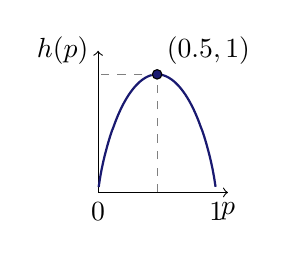
\begin{tikzpicture}[scale=1.5]
  \draw[->] (0,0) -- (1.1,0) node[below] {$p$};
  \draw[->] (0,0) -- (0,1.2) node[left]  {$h(p)$};
  \draw[domain=0.005:0.995, smooth, samples=80, thick, MidnightBlue]
    plot (\x, {-\x*ln(\x)/ln(2)-(1-\x)*ln(1-\x)/ln(2)});
  \draw[dashed, gray] (0.5,0) -- (0.5,1) -- (0,1);
  \draw[fill=MidnightBlue] (0.5,1) circle (0.04) node[above right] {$(0.5,1)$};
  \node[below] at (0,0) {$0$};
  \node[below] at (1,0) {$1$};
\end{tikzpicture}
\end{center}
\end{example}

二元信源是信息论中最基本的信源模型。$h(p)$ 曲线直观地说明：当两个符号等概时，最不确定，熵最大；当一个符号极大概率出现时，不确定性急剧下降。

\subsubsection*{$h(p)$ 的计算与常用值}

\textbf{计算方式}：$h(p)=-p\log_2 p-(1-p)\log_2(1-p)$。\\
若手头无计算器，可先将 $p$ 化为分数，利用 $\log_2\frac{a}{b}=\log_2 a-\log_2 b$ 分步计算。例如 $h(0.2)=h(\frac{1}{5})=-\frac{1}{5}\log_2\frac{1}{5}-\frac{4}{5}\log_2\frac{4}{5}$，其中 $\log_2\frac{1}{5}=-\log_2 5\approx -2.322$，$\log_2\frac{4}{5}=2-\log_2 5\approx -0.322$。

\textbf{利用对称性}：$h(p)=h(1-p)$，只需记住 $p\le 0.5$ 的一半即可。

\begin{center}
{\small
\begin{tabular}{c|cccccccccc}
\toprule
$p$    & 0     & 0.1   & 0.2   & 0.3   & 0.4   & 0.5 \\
\midrule
$h(p)$ & 0     & 0.469 & 0.722 & 0.881 & 0.971 & 1.000 \\
$p$    & 1.0   & 0.9   & 0.8   & 0.7   & 0.6   & --- \\
$h(p)$ & 0     & 0.469 & 0.722 & 0.881 & 0.971 & --- \\
\bottomrule
\end{tabular}
}
\end{center}

\noindent 考试中直接查表代入，可大幅节省计算时间。

\subsubsection{联合熵}
\begin{definitionBox}{联合熵}
二维随机变量 $(X,Y)$ 的联合熵为
\[
H(X,Y) = -\sum_{x}\sum_{y} p(x,y) \log p(x,y).
\]
\end{definitionBox}

联合熵衡量的是两个随机变量合在一起的整体不确定性。若 $X$ 与 $Y$ 独立，则 $H(X,Y)=H(X)+H(Y)$。

\noindent \textbf{使用说明}：联合熵有两种计算路径——\\[2pt]
路径 A（定义法）：$H(X,Y)=-\sum_{x,y}p(x,y)\log p(x,y)$，适用于已有完整联合分布表的情况，直接对表中所有非零概率项求和即可；\\
路径 B（链式法）：$H(X,Y)=H(X)+H(Y\mid X)=H(Y)+H(X\mid Y)$，适用于已算出边缘熵和条件熵的情况。\\
若 $X$ 与 $Y$ 独立则直接用 $H(X)+H(Y)$，无需重算联合分布。

\begin{example}
\textbf{联合熵的计算}：设 $(X,Y)$ 的联合分布如下表，求 $H(X,Y)$、$H(X)$、$H(Y)$ 和 $H(Y\mid X)$，并验证链式法则。

\begin{center}
\begin{tabular}{c|cc|c}
\toprule
$p(x,y)$ & $y=0$ & $y=1$ & $p(x)$ \\
\midrule
$x=0$ & $1/2$ & $1/8$ & $5/8$ \\
$x=1$ & $1/8$ & $1/4$ & $3/8$ \\
\midrule
$p(y)$ & $5/8$ & $3/8$ & $1$ \\
\bottomrule
\end{tabular}
\end{center}

\noindent \textbf{解题流程}：\\[2pt]
步骤一：直接代定义算 $H(X,Y)$——对联合分布中 4 个非零项分别算 $p\log p$ 再求和。\\
步骤二：从联合分布求边缘分布 $p(x)$ 和 $p(y)$（已在表格右侧与底部给出）。\\
步骤三：算 $H(X)=h(5/8)$，$H(Y)=h(5/8)$（借用 $h(p)$ 查表得 $h(0.625)\approx0.954$）。\\
步骤四：用链式法则 $H(Y\mid X)=H(X,Y)-H(X)$ 验证。

\textbf{解}：\\[2pt]
$H(X,Y)=-\frac{1}{2}\log_2\frac{1}{2}-\frac{1}{8}\log_2\frac{1}{8}-\frac{1}{8}\log_2\frac{1}{8}-\frac{1}{4}\log_2\frac{1}{4}
        =\frac{1}{2}\cdot1+\frac{1}{8}\cdot3+\frac{1}{8}\cdot3+\frac{1}{4}\cdot2=1.75$ bit。\\[2pt]
$H(X)=h(5/8)=h(0.625)\approx0.954$ bit，同理 $H(Y)=0.954$ bit。\\[2pt]
$H(Y\mid X)=H(X,Y)-H(X)=1.75-0.954=0.796$ bit。\\[2pt]
验证：$H(X,Y)=0.954+0.796=1.75$，与直接计算结果一致。
\end{example}

\subsubsection{条件熵}
\begin{definitionBox}{条件熵}
在给定 $Y$ 的条件下，$X$ 的条件熵为
\[
H(X \mid Y) = \sum_{y} p(y)\, H(X \mid Y=y)
            = -\sum_{x}\sum_{y} p(x,y) \log p(x \mid y).
\]
\end{definitionBox}

\begin{keypoint}{条件熵的含义}
$H(X \mid Y)$ 是已知 $Y$ 后，$X$ 尚存的\textbf{平均不确定性}。
\end{keypoint}

\noindent \textbf{使用说明}：条件熵的计算有两种常用路径——\\[2pt]
路径 A（定义法）：$H(X\mid Y)=-\sum_{x,y}p(x,y)\log p(x\mid y)$，适合已有完整联合分布表；\\
路径 B（期望法）：$H(X\mid Y)=\sum_{y}p(y)\cdot H(X\mid Y=y)$，适合按 $Y$ 的取值分组计算，如「三个盒子问题」。\\
建议先判断数据结构再选路径，路径 B 在考试中通常更省步骤。

\begin{formulaBox}{熵之间的基本关系}
\begin{align*}
  H(X,Y) &= H(X) + H(Y \mid X) = H(Y) + H(X \mid Y), \\
  H(Y \mid X) &= H(X,Y) - H(X), \\
  H(X \mid Y) &\le H(X).
\end{align*}
\end{formulaBox}

\begin{center}
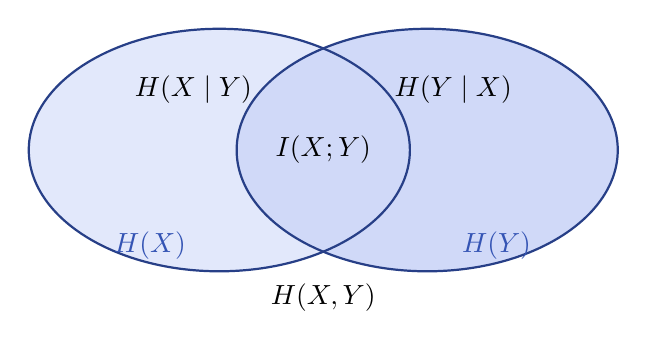
\begin{tikzpicture}[scale=1.1]
  % Left ellipse H(X)
  \fill[RoyalBlue!15]  (-1.2,0) ellipse (2.2 and 1.4);
  \fill[RoyalBlue!25]  ( 1.2,0) ellipse (2.2 and 1.4);
  \draw[RoyalBlue!60!black, thick] (-1.2,0) ellipse (2.2 and 1.4);
  \draw[RoyalBlue!60!black, thick] ( 1.2,0) ellipse (2.2 and 1.4);
  % Labels
  \node[RoyalBlue!80!black] at (-2.0, -1.1) {$H(X)$};
  \node[RoyalBlue!80!black] at ( 2.0, -1.1) {$H(Y)$};
  \node at (-1.5, 0.7) {$H(X \mid Y)$};
  \node at ( 1.5, 0.7) {$H(Y \mid X)$};
  \node at ( 0,   0)   {$I(X;Y)$};
  \node at ( 0,  -1.7) {$H(X,Y)$};
\end{tikzpicture}
\end{center}

上述三式是信息论中最常用的恒等变形关系，常被称为「熵的 Venn 图关系」——因为它们可以用两个相交椭圆来直观表示。开卷考试中，记住这三条等式可以大幅简化计算。

\subsubsection{相对熵}
\begin{definitionBox}{相对熵（KL 散度）}
两个分布 $P$ 和 $Q$ 之间的相对熵定义为
\[
\KL(P\|Q) = \sum_x P(x) \log \frac{P(x)}{Q(x)}.
\]
\end{definitionBox}

\begin{theoremBox}{相对熵的非负性}
$\KL(P\|Q) \ge 0$，等号成立当且仅当 $P=Q$。
\end{theoremBox}

\begin{keypoint}{相对熵的含义}
$\KL(P\|Q)$ 衡量用分布 $Q$ 近似真实分布 $P$ 时所需的额外信息量，也即两个分布之间的距离度量。
\end{keypoint}

\begin{example}
\textbf{KL 散度计算}（相对熵的计算）：设真实分布 $P=(0.5,0.5)$，近似分布 $Q=(0.25,0.75)$，求 $\KL(P\|Q)$。

\noindent \textbf{解题流程}：\\[2pt]
步骤一：明确方向——$\KL(P\|Q)$ 表示用 $Q$ 近似 $P$ 的代价，先写 $P$ 再写 $Q$，底数取 2。\\
步骤二：逐项计算——对每个 $x$，算 $P(x)\log_2\frac{P(x)}{Q(x)}$。\\
步骤三：求和——两项相加即得最终结果。

\textbf{解}：\\[2pt]
\[
\KL(P\|Q)=0.5\log_2\frac{0.5}{0.25}+0.5\log_2\frac{0.5}{0.75}\approx 0.208\text{ bit}.
\]

注意 $\KL(P\|Q)$ 不是对称的：一般来说 $\KL(P\|Q) \neq \KL(Q\|P)$，所以它不是真正意义上的「距离」，但可以看作一种有向的差异度量。它在线性模型、机器学习变分推断等领域有广泛应用。
\end{example}

\subsection{信息熵的基本性质}

熵不仅仅是一个计算公式，它具备一系列优美的数学性质，这些性质在推导和证明中经常用到。理解每条性质的\textbf{物理含义}比死记符号更有用。

\begin{theoremBox}{信息熵的基本性质}
信息熵 $H(X)$ 具有以下性质：
\begin{enumerate}
  \item \textbf{对称性}：$H(p_1,\dots,p_n)=H(p_{\sigma(1)},\dots,p_{\sigma(n)})$；
  \item \textbf{非负性}：$H(X) \ge 0$；
  \item \textbf{确定性}：若某个 $p_i=1$，则 $H(X)=0$；
  \item \textbf{扩展性}：$H(p_1,\dots,p_n,0)=H(p_1,\dots,p_n)$；
  \item \textbf{可加性}：$H(X,Y)=H(X)+H(Y \mid X)$；
  \item \textbf{链原则}：$H(X_1,\dots,X_n)=\sum_{i=1}^{n}H(X_i \mid X_1,\dots,X_{i-1})$；
  \item \textbf{极值性}：$H(X) \le \log n$，等号成立当且仅当等概；
  \item \textbf{上凸性}：$H(p)$ 是 $p$ 的上凸函数。
\end{enumerate}
\end{theoremBox}

\noindent 简记口诀：\textbf{对、非、确、扩、加、链、极、凸}。\\
其中\textbf{极值性}和\textbf{上凸性}在后续信道容量和率失真函数推导中会反复用到，是本章最重要的两条性质。

\begin{methodBox}{熵的计算与比较}
\begin{enumerate}
  \item 判断信源类型：离散无记忆？马尔可夫？
  \item 写出概率分布表；
  \item 使用链则或定义直接计算；
  \item 验证结果的合理性：$0 \le H \le \log n$。
\end{enumerate}
\end{methodBox}

\begin{example}
\textbf{三个盒子问题}（条件熵的计算）：有三个盒子。盒 1 有 2 红 8 白，盒 2 有 5 红 5 白，盒 3 有 8 红 2 白。等概率随机选择一个盒子，再从中摸一个球。设 $X$ 为盒子编号，$Y$ 为球的颜色。比较 $H(X)$、$H(Y)$、$H(Y \mid X)$。

\noindent \textbf{解题流程}：\\[2pt]
步骤一：分析数据结构。$X$ 是盒子编号，等概——直接代 $H(X)=\log n$。\\
步骤二：算条件熵——用路径 B（期望法）：$H(Y\mid X)=\frac{1}{3}[h(0.2)+h(0.5)+h(0.8)]$。\\
步骤三：算 $H(Y)$——先通过全概率公式求 $p(y)$，再代熵的定义。\\
步骤四：验证——$H(Y\mid X) < H(Y)$ 应成立（条件降低不确定性）。

\textbf{解}：\\
$X$ 等概取三个值，故 $H(X)=\log_2 3 \approx 1.585$ bit。\\
已知盒子后，摸球的不确定性来自该盒内红白比例：\\
盒 1：$H(Y\mid X=1)=h(0.2)\approx 0.722$，盒 2：$H(Y\mid X=2)=h(0.5)=1$，盒 3：$H(Y\mid X=3)=h(0.8)\approx 0.722$。\\
$H(Y\mid X)=\frac{1}{3}(0.722+1+0.722)\approx 0.815$ bit。\\
$H(Y)$ 需先求 $Y$ 的边缘分布。由全概率公式：\\[2pt]
$P(Y=\text{红}) = \frac{1}{3}(0.2+0.5+0.8)=\frac{1.5}{3}=0.5$，
$P(Y=\text{白}) = 1-0.5=0.5$。\\[2pt]
因此 $H(Y)=h(0.5)=1$ bit。\\[2pt]
验证：$H(Y\mid X)=0.815 < H(Y)=1$，条件确实降低了不确定性，符合预期。
\end{example}

\begin{example}
\textbf{熵的比较}（熵的极值性）：比较甲、乙两城市天气的熵。甲：$(\frac{1}{2},\frac{1}{4},\frac{1}{4})$，乙：$(\frac{1}{3},\frac{1}{3},\frac{1}{3})$。

\noindent \textbf{解题流程}：\\[2pt]
步骤一：分别列出两个分布，确认概率和为 1。\\
步骤二：代熵的定义计算——甲直接算三项，乙由于等概可直接用 $\log_2 n$。\\
步骤三：比较数值并解释——熵大的一方不确定性更高，验证极值性：等概时熵最大。

\textbf{解}：\\[2pt]
甲：$H_1 = H(0.5,0.25,0.25)=1.5$ bit。\\
乙：$H_2 = H(\frac{1}{3},\frac{1}{3},\frac{1}{3})=\log_2 3\approx 1.585$ bit。\\[2pt]
乙城市天气分布更均匀，不确定性更大，天气预报「更有价值」——这正是极值性的直接体现。
\end{example}

\begin{warningBox}{最大熵与等概}
均匀分布对应最大熵，但实际计算中要注意概率和是否为 1，以及将零概率事件排除。
\end{warningBox}

\subsection{平均互信息}

\begin{remarkBox}{公式怎么选}
已知完整联合分布时，优先用 $I(X;Y)=H(X)+H(Y)-H(X,Y)$；已知信道矩阵和输入分布时，优先用 $I(X;Y)=H(Y)-H(Y\mid X)$。目标永远是选最省步骤的那条路。
\end{remarkBox}

前面 $I(x;y)$ 是事件层面的互信息，取决于具体取到的值，可能为正也可能为负。系统分析里更常用的是它的平均值，也就是平均互信息 $I(X;Y)$。

\subsubsection{平均互信息的定义}
\begin{definitionBox}{平均互信息}
随机变量 $X$ 与 $Y$ 之间的平均互信息为互信息的数学期望：
\[
I(X;Y) = \sum_{x,y} p(x,y) \log \frac{p(x,y)}{p(x)p(y)}.
\]
\end{definitionBox}

\begin{keypoint}{平均互信息含义}
$I(X;Y)$ 表示从 $Y$ 平均获得关于 $X$ 的信息量，也就是 $X$ 与 $Y$ 之间共享的信息。
\end{keypoint}

\subsubsection{平均互信息与熵的关系}
\begin{formulaBox}{平均互信息和熵的关系}
\begin{align*}
  I(X;Y) &= H(X) - H(X \mid Y), \\
  I(X;Y) &= H(Y) - H(Y \mid X), \\
  I(X;Y) &= H(X) + H(Y) - H(X,Y).
\end{align*}
\end{formulaBox}

\noindent \textbf{使用说明}——如何选择公式：\\[2pt]
\begin{itemize}
  \item 已知 $p(x,y)$ 完整联合分布时，用 $I = H(X)+H(Y)-H(X,Y)$ 最直接；
  \item 已知信道（$p(y\mid x)$）和输入分布（$p(x)$）时，用 $I = H(Y)-H(Y\mid X)$ 最方便；
  \item 已知 $p(x)$ 和 $p(x\mid y)$ 时，用 $I = H(X)-H(X\mid Y)$。\\
\end{itemize}
实质：三个公式完全等价，选哪个取决于你手头已知哪些量。

\subsubsection{平均互信息的性质}

平均互信息具备对称性、非负性等良好性质。其中\textbf{凸性}在信道容量计算中至关重要：它保证了我们可以用凸优化方法找到容量。

\begin{theoremBox}{平均互信息的性质}
\begin{enumerate}
  \item \textbf{对称性}：$I(X;Y)=I(Y;X)$；
  \item \textbf{非负性}：$I(X;Y) \ge 0$，等号当且仅当 $X$ 与 $Y$ 独立；
  \item \textbf{上界}：$I(X;Y) \le \min\{\,H(X),H(Y)\,\}$；
  \item \textbf{凸性}：固定 $p(y\mid x)$，$I(X;Y)$ 是 $p(x)$ 的上凸函数；\\
        \hspace*{2em} 固定 $p(x)$，$I(X;Y)$ 是 $p(y\mid x)$ 的下凸函数。
\end{enumerate}
\end{theoremBox}

\noindent 凸性的直观理解：\\
固定信道（$p(y\mid x)$）时，输入越均匀，互信息越大（上凸，存在最大值即为信道容量）；\\
固定输入时，信道越「纯净」，互信息越大。这正是香农第二定理中信道容量的数学基础。

\begin{methodBox}{平均互信息的计算}
\begin{enumerate}
  \item 写出联合分布 $p(x,y)$ 或给定信道矩阵和输入分布；
  \item 求边缘分布 $p(x)$、$p(y)$；
  \item 选择最短路径：\\
    路径一：$I = H(X) - H(X\mid Y)$；\\
    路径二：$I = H(Y) - H(Y\mid X)$；\\
    路径三：$I = H(X) + H(Y) - H(X,Y)$；
  \item 验算：$I(X;Y)$ 应为非负数。
\end{enumerate}
\end{methodBox}
\subsubsection{平均条件互信息}

当系统中存在多个变量时，我们常需要计算在已知某个变量的条件下，另外两个变量之间的互信息。这在多用户信息论和网络信息论中非常常见。

\begin{definitionBox}{平均条件互信息}
在给定 $Z$ 的条件下，$X$ 与 $Y$ 的平均条件互信息为
\[
I(X;Y \mid Z) = H(X \mid Z) - H(X \mid Y,Z).
\]
\end{definitionBox}
\subsubsection{平均互信息的链原则}

链式法则告诉我们：多个变量联合提供给 $Y$ 的信息，等于逐个变量在已知前面变量之后提供的条件互信息之和。这和熵的链式法则在形式上完全对应。

\begin{theoremBox}{链式法则（互信息）}
\[
I(X_1,X_2,\dots,X_n;Y) = \sum_{i=1}^{n} I(X_i;Y \mid X_1,\dots,X_{i-1}).
\]
\end{theoremBox}

% ========== 题型整理：平均互信息 ==========
\subsubsection{题型整理：平均互信息的计算与应用}

\noindent \textbf{信道矩阵的写法}：\\[2pt]
信道矩阵即条件概率矩阵 $P(Y\mid X)$，是分析信道问题的核心工具。\\
构造规则：
\begin{itemize}
  \item \textbf{行}对应输入 $X$，\textbf{列}对应输出 $Y$，元素为 $p(y\mid x)$；
  \item \textbf{每行和为 1}（给定输入，所有输出的条件概率之和必为 1）；
  \item 矩阵大小：输入符号数 $\times$ 输出符号数。
\end{itemize}
例如 BSC（二元对称信道）：输入 $\{0,1\}$、输出 $\{0,1\}$，错误概率 $\varepsilon$。第 0 行表示输入为 0 时正确传为 0 的概率为 $1-\varepsilon$、错误翻为 1 的概率为 $\varepsilon$。写成矩阵：
\[
P(Y\mid X) = \begin{pmatrix}
1-\varepsilon & \varepsilon \\
\varepsilon    & 1-\varepsilon
\end{pmatrix}
\quad\text{（行和为 1：$(1-\varepsilon)+\varepsilon=1$）}.
\]
已知信道矩阵和输入分布 $p(x)$ 后，输出分布通过全概率公式得到：$p(y)=\sum_x p(x)\,p(y\mid x)$。

\begin{hintBox}{信道题读题顺序}
信道题通常按“输入分布 $p(x)$ $\to$ 信道矩阵 $p(y\mid x)$ $\to$ 输出分布 $p(y)$ $\to$ 互信息”的顺序做。不要一上来就套互信息公式，先把输入、信道、输出三层关系理清。
\end{hintBox}

\begin{example}
\textbf{二元对称信道}（平均互信息的计算）：输入 $X$ 等概（$p(0)=p(1)=0.5$），错误概率 $\varepsilon$。
\begin{enumerate}
  \item 写出信道矩阵 $P(Y\mid X)$；
  \item 计算 $H(Y)$、$H(Y\mid X)$；
  \item 求平均互信息 $I(X;Y)$。
\end{enumerate}

\noindent \textbf{解题流程}：\\[2pt]
步骤一：写信道矩阵。BSC 是标准矩阵，每行和为 1，对角线为 $1-\varepsilon$，反对角线为 $\varepsilon$。\\
步骤二：求输出分布。用 $p(y)=\sum_x p(x)p(y\mid x)$。当输入等概、信道对称时，输出也等概——这是一个可以直接用的结论。\\
步骤三：算条件熵。$H(Y\mid X)$ 是每行熵的加权平均。由于每行相同，直接 $H(Y\mid X)=h(\varepsilon)$。\\
步骤四：用 $I=H(Y)-H(Y\mid X)$ 得出结果。最后代入 $\varepsilon$ 的边界值验证：$\varepsilon=0$ 时 $I=1$，$\varepsilon=0.5$ 时 $I=0$。

\textbf{解}：\\
(1) 信道矩阵为
\[
P(Y\mid X) = \begin{pmatrix}
1-\varepsilon & \varepsilon \\
\varepsilon    & 1-\varepsilon
\end{pmatrix}.
\]
(2) 由输入等概可得输出也是等概：$p(0)=p(1)=0.5$，故 $H(Y)=1$ bit。\\
条件熵 $H(Y\mid X) = h(\varepsilon) = -\varepsilon\log\varepsilon-(1-\varepsilon)\log(1-\varepsilon)$。\\
(3) $I(X;Y)=H(Y)-H(Y\mid X)=1-h(\varepsilon)$。\\[2pt]
当 $\varepsilon=0$（无误码）时，$I=1$ bit，信道完美传输信息；\\
当 $\varepsilon=0.5$（完全随机）时，$I=0$ bit，信道无法传输任何信息。

\begin{center}
\begin{tikzpicture}[>=stealth, node distance=2.5cm, scale=1.1]
  \node[circle, draw, thick, fill=RoyalBlue!10] (x0) at (0,1.5) {$0$};
  \node[circle, draw, thick, fill=RoyalBlue!10] (x1) at (0,0)   {$1$};
  \node[circle, draw, thick, fill=Orange!10]   (y0) at (2.5,1.5) {$0$};
  \node[circle, draw, thick, fill=Orange!10]   (y1) at (2.5,0)   {$1$};
  \node at (0, -0.6)  {$X$（输入）};
  \node at (2.5, -0.6){$Y$（输出）};
  \draw[->, thick, MidnightBlue] (x0) -- (y0) node[midway, above] {$1-\varepsilon$};
  \draw[->, thick, red!60]       (x0) -- (y1) node[midway, sloped, above] {$\varepsilon$};
  \draw[->, thick, red!60]       (x1) -- (y0) node[midway, sloped, below] {$\varepsilon$};
  \draw[->, thick, MidnightBlue] (x1) -- (y1) node[midway, below] {$1-\varepsilon$};
\end{tikzpicture}
\end{center}
\end{example}

\begin{example}
\textbf{二元删除信道}（平均互信息的计算）：输入 $X$ 等概（$p(0)=p(1)=0.5$），输出 $Y \in \{0,?,1\}$。信道以概率 $p$ 将输入符号变为「?」（删除），以概率 $1-p$ 正确传输。

\begin{enumerate}
  \item 写出信道矩阵 $P(Y\mid X)$；
  \item 计算 $H(Y)$ 和 $I(X;Y)$。
\end{enumerate}

\noindent \textbf{解题流程}：\\[2pt]
步骤一：写信道矩阵——输入 2 个符号、输出 3 个符号，矩阵为 $2\times3$，正确传输在对角，删除列在中间。\\
步骤二：求输出分布——用 $p(y)=\sum_x p(x)p(y\mid x)$，利用对称性简化。\\
步骤三：算条件熵——$H(Y\mid X)=h(p)$（原因同 BSC：每行相同，直接取一行算）。\\
步骤四：算互信息——$I=H(Y)-H(Y\mid X)$，最后与 BSC 对比。

\textbf{解}：\\[2pt]
(1) 信道矩阵为
\[
P(Y\mid X) = \begin{pmatrix}
1-p & p & 0 \\
0   & p & 1-p
\end{pmatrix}.
\]
(2) 由输入等概及信道对称性，$p_Y(0)=p_Y(1)=\frac{1-p}{2}$，$p_Y(?)=p$。\\
$H(Y)=-(1-p)\log\frac{1-p}{2}-p\log p = (1-p)(1+\log\frac{1}{1-p})+p\log\frac{1}{p}$。\\
条件熵 $H(Y\mid X)=h(p)$（给定输入后，输出不确定性仅来自删除概率）。\\
因此 $I(X;Y)=H(Y)-H(Y\mid X)=1-p$ bit。\\[2pt]
比较：对于相同的错误概率 $p$，删除信道的互信息\textbf{高于}对称信道——因为删除信道明确告诉你「我不知道」，而不是给你错误答案。
\end{example}

\begin{formulaBox}{数据处理不等式}
若 $X \to Y \to Z$ 构成 Markov 链，则
\[
I(X;Z) \le I(X;Y), \qquad I(X;Z) \le I(Y;Z).
\]

\begin{center}
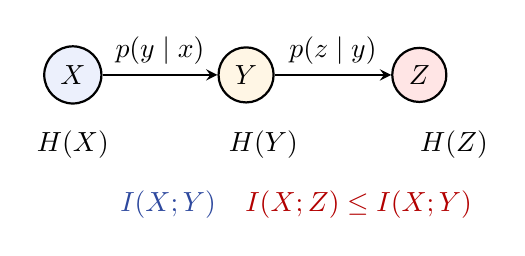
\begin{tikzpicture}[>=stealth, node distance=2.2cm, scale=1.1]
  \node[circle, draw, thick, fill=RoyalBlue!10] (X) {$X$};
  \node[circle, draw, thick, fill=Orange!10]   (Y) [right of=X] {$Y$};
  \node[circle, draw, thick, fill=Red!10]      (Z) [right of=Y] {$Z$};
  \draw[->, thick] (X) -- (Y) node[midway, above] {$p(y\mid x)$};
  \draw[->, thick] (Y) -- (Z) node[midway, above] {$p(z\mid y)$};
  \node at (0, -0.8)    {$H(X)$};
  \node at (2.2, -0.8)  {$H(Y)$};
  \node at (4.4, -0.8)  {$H(Z)$};
  \node[RoyalBlue!70!black] at (1.1, -1.5)  {$I(X;Y)$};
  \node[red!70!black]      at (3.3, -1.5)  {$I(X;Z) \le I(X;Y)$};
\end{tikzpicture}
\end{center}

该不等式的物理含义：\textbf{对数据的任何处理都不会增加信息量}。无论你对收到的信号 $Y$ 做什么后处理（如解码、滤波、压缩），关于原始信号 $X$ 的信息只会减少或不变，绝不会凭空增加。
这也是为什么在通信系统里，我们总是先尽量保留信息，再做处理，而不是指望后处理“补回”丢掉的信息。
\end{formulaBox}

\begin{warningBox}{常见混淆}
不要混淆：
\begin{itemize}
  \item $I(x;y)$（事件层面互信息，可为负）与 $I(X;Y)$（平均互信息，非负）；
  \item $H(X \mid Y)=0$（$Y$ 完全决定 $X$）与 $I(X;Y)=0$（平均意义下 $X$ 与 $Y$ 独立）；
  \item 互信息的对称性：$I(X;Y)=I(Y;X)$，这是很多公式推导的出发点。
\end{itemize}
\end{warningBox}

\subsection{公式速查表}

{\scriptsize
\begin{tabularx}{\textwidth}{@{}l>{\raggedright\arraybackslash}X>{\raggedleft\arraybackslash}p{1.8em}@{}}
\toprule
\textbf{类别} & \textbf{公式} & \textbf{编号} \\
\midrule
自信息 & $I(x)=-\log p(x)$ & (1) \\
联合自信息 & $I(x,y)=-\log p(x,y)$ & (2) \\
条件自信息 & $I(x\mid y)=-\log p(x\mid y)$ & (3) \\
\textcolor{Red}{互信息} & $\textcolor{Red}{I(x;y)=\log\frac{p(x\mid y)}{p(x)}=I(x)-I(x\mid y)}$ & (4) \\
自信息关系 & $I(x,y)=I(x)+I(y\mid x)$ & (5) \\
互信息对称性 & $I(x;y)=I(y;x)=\log\frac{p(x,y)}{p(x)p(y)}$ & (6) \\
\midrule
\textcolor{Red}{信息熵} & $\textcolor{Red}{H(X)=-\sum_x p(x)\log p(x)}$ & (7) \\
二元熵 & $h(p)=-p\log p-(1-p)\log(1-p)$ & (8) \\
联合熵 & $H(X,Y)=-\sum_{x,y}p(x,y)\log p(x,y)$ & (9) \\
条件熵 & $H(X\mid Y)=\sum_y p(y)H(X\mid Y=y)$ & (10) \\
\midrule
\textcolor{Red}{熵的关系} & $\textcolor{Red}{H(X,Y)=H(X)+H(Y\mid X)}$ & (11) \\
 & $H(X\mid Y)\le H(X)$ & (12) \\
 & $0\le H(X)\le\log|\mathcal{X}|$ & (13) \\
\midrule
相对熵 & $\textcolor{Red}{\KL(P\|Q)=\sum_x P(x)\log\frac{P(x)}{Q(x)}\ge 0}$ & (14) \\
\midrule
\textcolor{Red}{平均互信息} & $I(X;Y)=\sum_{x,y}p(x,y)\log\frac{p(x,y)}{p(x)p(y)}$ & (15) \\
 & $\textcolor{Red}{I(X;Y)=H(X)-H(X\mid Y)=H(Y)-H(Y\mid X)}$ & (16) \\
 & $\textcolor{Red}{\;\,\qquad=H(X)+H(Y)-H(X,Y)}$ & (17) \\
 & $I(X;Y)\ge 0$，$I(X;Y)\le\min\{H(X),H(Y)\}$ & (18) \\
条件互信息 & $I(X;Y\mid Z)=H(X\mid Z)-H(X\mid Y,Z)$ & (19) \\
\midrule
\textcolor{Red}{熵的链则} & $H(X_1^n)=\sum_{i=1}^{n}H(X_i\mid X_1^{i-1})$ & (20) \\
\textcolor{Red}{互信息链则} & $I(X_1^n;Y)=\sum_{i=1}^{n}I(X_i;Y\mid X_1^{i-1})$ & (21) \\
\midrule
\textcolor{Red}{数据处理不等式} & $\textcolor{Red}{X\!\to\!Y\!\to\!Z\;\Rightarrow\;I(X;Z)\le I(X;Y)}$ & (22) \\
\bottomrule
\end{tabularx}
}

\subsection{本章要求}
\begin{remarkBox}{第二章学习重点}
\begin{itemize}
  \item \textbf{自信息}和\textbf{互信息}的定义与计算（注意对数的底）；
  \item \textbf{信息熵}的定义、性质和计算（尤其二元信源 $h(p)$）；
  \item \textbf{联合熵}、\textbf{条件熵}的关系链及计算；
  \item \textbf{相对熵}的定义与非负性；
  \item \textbf{平均互信息}与熵的转换关系，以及凸性性质；
  \item 常见题型：摸球、棋盘、二元信道等经典问题的计算流程。
\end{itemize}
\end{remarkBox}
